\pdfobjcompresslevel=0
\pdfminorversion=4




\documentclass[english,10pt]{article}
\usepackage{graphicx}
\usepackage{babel}
\usepackage{graphics}
\usepackage{setspace}
\usepackage{paralist}
\usepackage{psfrag}
\usepackage{latexsym}
\usepackage{amssymb}
\usepackage{amsmath}
\usepackage{caption}
\usepackage{amsfonts}
\usepackage{multirow}
\usepackage{amsmath}
\usepackage{epsfig}
\usepackage{mathrsfs}
\usepackage{geometry}
\usepackage{rotating}
\usepackage{subcaption}
%ts_st
% \usepackage{algorithm}
%ts_end

\usepackage{adjustbox}
\usepackage[noend]{algpseudocode}
\usepackage[hyphens]{url}
\usepackage{times}
\usepackage{latexsym}
\usepackage{graphicx}
\usepackage{tikz}
\usepackage{tikz-cd}
\usepackage{subcaption}
\usepackage{multirow}
\usepackage{amsmath}
%\usepackage[export]{adjustbox}
\usepackage{tabularx}
\usepackage{enumitem}
\usepackage{tikz}
\usepackage{tikz-cd}
\usepackage{array}
% ts_st
% \usepackage{algorithm, algpseudocode}
\usepackage{algorithm2e}
%ts_end
\usepackage{multirow}
\usepackage{booktabs}
\usepackage{footmisc}
\usepackage{booktabs} % For formal tables
\usepackage{todonotes}
\usepackage{subcaption}
\usepackage{colortbl}
\usepackage{color}
\usepackage{tcolorbox}
\usepackage[hidelinks]{hyperref}

\usepackage[numbers]{natbib}

\newcommand{\citetest}[1]
{\citeauthor{#1}\shortcite{#1}}
\newcommand{\zij}{z_{ij}}
\newcolumntype{M}[1]{>{\centering\arraybackslash}m{#1}}
\newcolumntype{N}{@{}m{0pt}@{}}
%\usepackage{csquotes}
\usepackage{url}
\usepackage{xkeyval}
%ts_start
\usepackage{amsmath,amssymb,amsfonts}
\usepackage{textcomp}
\usepackage{xcolor}
\usepackage{tikz}
\usepackage{subcaption}
\usepackage{rotating}
\usepackage{pgfplots}
%\usepackage[margin=3cm]{geometry}
%ts_end
%\usepackage{mdframed}
\usepackage{booktabs} % For formal tables

\PassOptionsToPackage{export}{adjustbox}

\geometry{verbose,a4paper,tmargin=2.54cm,bmargin=2.54cm,lmargin=2.54cm,rmargin=2.54cm}
\linespread{1.5}

% Project figures live in Figures/; experiment plots are generated under ../graphs/
\graphicspath{{Figures/}{../graphs/}}

\begin{document}
\thispagestyle{empty}
\begin{titlepage}
\begin{center}
    \vspace*{0.5in}
    {\huge\textbf{Multipath Transport in Heterogeneous Networks:}} \\
    \vspace{0.15in}
    {\huge\textbf{MPTCP vs.\ TCP Under Mobility and Path Failures}} \\
    \vspace{0.6in}
     {\Large\bf Internet Architecture and Protocols Term Project Report }\\
     
    \vspace{0.4in}
    {\Large\bf Internet Architecture and Protocols (CS60008)}\\
    \vspace{0.35in}
    {\Large\bf by}\\
    \vspace{0.25in}
    
    {\large\bf Navaneeth Shaji (21CS30032)}\\
    \vspace{0.12in}
    {\large\bf Vikyath Gummadi (21CS30070)}\\
    \vspace{0.12in}
    {\large\bf Kalal Bhavani (21CS30027)}\\
    \vspace{0.5in}
    
    \vspace{0.3in}
    \begin{center}
        
\includegraphics[width=1.2in]{Figures/iitkgp_logo.png}
    \end{center}
    {\Large\textbf{Department of Computer Science and Engineering,}}\medskip\\
    {\Large\textbf{Indian Institute of Technology Kharagpur}}\medskip\\
    {\large\textbf{April 2026}}
\end{center}
\end{titlepage}

\setcounter{page}{2}
% \newpage
% \input{Front_Matter/certificate.tex}
% \newpage
% \input{Front_Matter/acknowledgement.tex}

\newpage
\begin{singlespace}
\tableofcontents
\newpage
\listoffigures
\newpage
% \listoftables
% \newpage

\section{Introduction}
\label{sec:intro}

Mobile and multihomed hosts often see several access networks at once (for example Wi-Fi and cellular). Regular TCP binds a connection to a single four-tuple, so a change of interface or loss of that path can interrupt the application unless higher layers recover. Multipath TCP (MPTCP) extends TCP so one logical connection may use several \emph{subflows} across different paths, with the goal of higher throughput when paths add capacity and smoother handover when one path disappears~\cite{rfc8684,Bonaventure2012usecases}.

This term project builds a small \emph{experimental framework} to compare baseline single-path TCP against a multipath-style setup under controlled link conditions. We use Mininet~\cite{Lantz2010mininet} with \texttt{TCLink} bandwidth and delay, Linux policy routing and kernel MPTCP endpoints where applicable, and \texttt{iperf3}~\cite{iperf3} with JSON output for throughput time series. Mobility-like events are \emph{emulated}: sudden interface down on one path, bandwidth collapse via \texttt{tc}, and RTT inflation via \texttt{netem}~\cite{linuxnetem}.

\textbf{Objectives} (aligned with the course project brief):
\begin{itemize}[noitemsep]
  \item Quantify per-path and combined throughput under heterogeneous caps and delays.
  \item Observe session continuity when one path is removed while traffic continues on another.
  \item Stress one path with bandwidth collapse and RTT spikes and compare aggregate behavior to single-path TCP.
  \item Discuss latency and scheduler effects qualitatively from throughput traces.
  \item Study a handover-like scenario by ramping RTT on the preferred path while a second path stays available (Experiment~6).
\end{itemize}
\textbf{Competing-flow fairness} in the sense of multiple independent flows sharing the same paths (e.g., Jain fairness with cross-traffic) is \emph{not} measured here; Experiment~6 instead reports scheduler and throughput behavior under primary-path degradation.

\textbf{Contributions of this report:} (i)~a reproducible Mininet-based workflow mapping six Python experiment drivers to measurement outputs; (ii)~numeric summaries from our captured logs (including tabular time-slice data where no figure is available); and (iii)~an honest discussion of limitations, including that our multipath measurements use parallel \texttt{iperf3} flows bound to interfaces as a practical stand-in for a single MPTCP socket in all scenarios.



\section{Related Work}
\label{sec:related_work}

Multipath TCP standardizes extensions to TCP so endpoints can advertise multiple addresses, add subflows, and schedule data across paths while presenting one byte stream to the application~\cite{rfc8684}. Early community discussion highlighted use cases such as smartphones combining Wi-Fi and cellular and the need for congestion control and fairness across coupled subflows~\cite{Bonaventure2012usecases}. Subsequent work has studied performance factors such as header compression interactions with multipath scheduling~\cite{Paasch2014experimental}.

Our work is \emph{emulation-based} rather than wide-area deployment: we borrow the problem framing from the MPTCP literature but evaluate under synthetic topologies. Closely related systems work includes Mininet for repeatable SDN and end-host experiments~\cite{Lantz2010mininet}, \texttt{iperf3} for transport throughput~\cite{iperf3}, and Linux \texttt{tc}/\texttt{netem} for link impairment~\cite{linuxnetem}. These tools match the assignment's suggested stack (Mininet and/or Linux traffic control).

\section{Preliminaries and Core Idea}
%\input{Main_Matter/JOI/preliminaries}
%\section{Motivation}
%\input{Main_Matter/JOI/motivation}

\section{Proposed Methodology}
\label{sec:proposed_architecture}

We follow a single evaluation pattern: deploy a two-path Mininet topology, configure addressing and routing, run \texttt{iperf3} clients and servers with \texttt{--json} and one-second intervals, parse interval throughput in megabits per second, and plot time series or bar summaries. Events are injected at a known time $t$ (typically $10$--$11$~s) so pre- and post-event windows are comparable.

\subsection{Topology and addressing}
Two Ethernet paths connect hosts \texttt{h1} and \texttt{h2}. Each host has two interfaces, each on a distinct subnet, emulating heterogeneous access (for example Wi-Fi-like vs.\ LTE-like, or two symmetric paths). Baseline TCP uses one destination IP at a time. Multipath experiments add a third ``logical'' subnet or use policy routing so replies exit the same interface that originated a subflow, which is required for correct subflow establishment.

\subsection{Experiment~1: Independent TCP baselines}
Run two sequential \texttt{iperf3} transfers from \texttt{h1} to \texttt{h2}, each bound to a single path, to establish per-path throughput near configured \texttt{TCLink} caps.

\subsection{Experiment~2: Parallel streams and aggregation}
After enabling MPTCP in the kernel and configuring endpoints, run \emph{two} concurrent \texttt{iperf3} clients, one bound to each interface, and compare the sum of average throughputs to the sum of the Experiment~1 TCP baselines. This measures how much capacity is usable when both paths are active simultaneously (aggregation), separate from single-socket MPTCP dynamics.

\subsection{Experiment~3: Path failure}
Start both parallel transfers for $30$~s. At $t=10$~s, administratively disable the receiver's interface on the first path (\texttt{ip link set} \ldots \texttt{down}), then terminate the corresponding client. The second stream continues, emulating sudden loss of one access network while the other remains.

\subsection{Experiment~4: Bandwidth collapse}
On a symmetric pair of $10$~Mb/s paths, run parallel streams for $25$~s. At $t=10$~s, reshape the second path to $2$~Mb/s using \texttt{tc} on host interfaces and switch ports. Record whether aggregate throughput is preserved by shifting load to the stable path.

\subsection{Experiment~5: RTT spike}
With two $10$~Mb/s paths and baseline RTT near $40$~ms, first run TCP only on the second path and inject a large one-way delay with \texttt{netem} at $t=10$~s (target RTT on the order of hundreds of milliseconds). Restore the link, then repeat under parallel two-path transfer. Compare single-path collapse to multipath resilience using combined throughput before and after the spike.

\subsection{Experiment~6: Handover via primary-path RTT ramp}
Two $10$~Mb/s paths with different baseline delays emulate a preferred fast path and a slower backup. After a dual-stream baseline, run parallel transfers for $25$~s and starting near $t=10$~s increase Path~1's delay in steps using \texttt{netem} on host interfaces and the Path~1 switch ports. The kernel MPTCP scheduler (we use \texttt{blest}) should prefer the lower-RTT path when possible and migrate traffic as Path~1 degrades. Outcomes are reported from \texttt{iperf3} interval sums and driver-computed before/after window averages (no separate PNG in our current pipeline).

\subsection{Metrics}
\textbf{Throughput} is taken from \texttt{iperf3} \texttt{end.sum\_received.bits\_per\_second} and per-interval arrays. \textbf{Session continuity} for path failure is evidenced by continued nonzero throughput on the surviving stream without restarting the server. \textbf{Resilience ratios} ``throughput retained (\%)'' are computed from average combined Mbps in defined pre- and post-event windows printed by our drivers. \textbf{Latency inflation} is imposed by \texttt{netem}; we interpret its effect indirectly via throughput and retransmissions rather than end-to-end RTT sampling in this report.

\section{Implementation}
\label{sec:implementation}

All experiments are implemented as standalone Python scripts (\texttt{1.py}--\texttt{6.py}) in the assignment repository root. Scripts \texttt{1.py}--\texttt{5.py} share \texttt{plot\_helpers.py}, which writes PNG figures into \texttt{../graphs/} when Matplotlib is available. \texttt{6.py} currently emits ASCII plots and numeric tables to the console only (see \texttt{Outputs/6.txt}).

\subsection{Mininet and links}
We construct custom \texttt{Topo} subclasses and instantiate \texttt{Mininet(..., link=TCLink, switch=OVSBridge, controller=None)}. Per-link bandwidth (Mb/s) and delay strings follow Mininet's \texttt{TCLink} conventions; RTT is approximately twice the one-way delay plus switching overhead.

\subsection{Experiment~\texttt{1.py}}
Hosts receive static \texttt{/24} addresses on each subnet. \texttt{run\_tcp\_baseline} starts \texttt{iperf3 -s} on \texttt{h2}, then runs two sequential clients from \texttt{h1} to \texttt{10.0.1.2} and \texttt{10.0.2.2}. Results are parsed with \texttt{json.loads} from the client stdout.

\subsection{Experiment~\texttt{2.py}}
Adds policy routing tables and rules so traffic sourced from each local address exits the matching interface. Kernel MPTCP is enabled (\texttt{sysctl net.mptcp.enabled=1}), and \texttt{ip mptcp endpoint add ... dev ...} advertises addresses. Part~2 repeats per-path TCP baselines; Part~3 launches two clients to distinct server ports, bound per interface, and records \texttt{ss} lines for established flows during the transfer.

\subsection{Experiment~\texttt{3.py}}
Uses the same MPTCP-oriented addressing as Experiment~2. Two clients run for $30$~s. At $t=10$~s the receiver's Wi-Fi-side interface is brought down; the Wi-Fi client is killed so JSON may be partial while the LTE JSON completes.

\subsection{Experiment~\texttt{4.py}}
Symmetric $10$~Mb/s paths. Part~1--2 mirror baselines and dual-stream aggregation. Part~3 applies \texttt{tc qdisc replace ... tbf} (and related) on path~2 interfaces and switch ports at $t=10$~s to emulate collapse to $2$~Mb/s.

\subsection{Experiment~\texttt{5.py}}
Same symmetric topology as Experiment~4 for baselines. Part~3 runs TCP only on path~2. Part~4 runs dual streams. \texttt{tc netem} adds $\approx 800$~ms one-way delay per hop on path~2 at $t=10$~s, then restores baseline \texttt{netem} delay after the run.

\subsection{Experiment~\texttt{6.py}}
Dual path with Path~1 at $20$~ms per link hop and Path~2 at $50$~ms (both $10$~Mb/s). Sets \texttt{net.mptcp.scheduler=blest}, policy routing, and MPTCP endpoints as in other multipath scripts. Part~1--2: TCP baselines and $15$~s dual-stream aggregation. Part~3: $25$~s parallel streams with \texttt{degrade\_path1\_for\_handover} stepping Path~1 \texttt{netem} delay ($100$--$250$~ms targets) on \texttt{h1}/\texttt{h2} \texttt{eth0} and \texttt{s1} OVS ports after $t\approx 10$~s.

\subsection{Reproducibility}
Run each script with appropriate privileges (Mininet typically requires root). Capture console logs to the \texttt{Outputs/} text files referenced in Section~\ref{sec:results}. Regenerate figures by ensuring Python~3 dependencies in \texttt{requirements.txt} are installed.

\section{Results and Discussions}
\label{sec:results}

All numbers below come from the captured logs in \texttt{Outputs/1.txt}--\texttt{Outputs/6.txt} unless noted. Figures are generated by the experiment scripts into \texttt{graphs/} where implemented. Where we use two parallel \texttt{iperf3} flows, combined throughput is the sum of per-flow averages or per-interval sums as printed by the driver.

\subsection{Limitations}
Parallel clients bound to interfaces approximate multipath capacity; they are not always identical to a single MPTCP connection ID in the kernel. Experiment~6 studies \emph{handover-like} behavior (primary-path RTT degradation) rather than Jain-fair bandwidth sharing among independent competing flows; the latter remains a possible extension (Section~\ref{sec:future}).

\subsection{Experiment~1: TCP per-path baselines}
Table~\ref{tab:exp1} summarizes independent TCP runs on each emulated path. Throughput sits close to the configured caps (10 and 20~Mb/s), indicating sane Mininet shaping.

\begin{table}[htbp]
  \centering
  \caption{Experiment~1: baseline TCP average throughput (10~s runs).}
  \label{tab:exp1}
  \begin{tabular}{lccc}
    \toprule
    Path & Config.\ cap & Avg.\ throughput & Retransmissions \\
    \midrule
    Path~1 (Wi-Fi-like) & 10~Mb/s & 9.45~Mb/s & 0 \\
    Path~2 (LTE-like)   & 20~Mb/s & 16.95~Mb/s & 0 \\
    \bottomrule
  \end{tabular}
\end{table}

\begin{figure}[htbp]
  \centering
  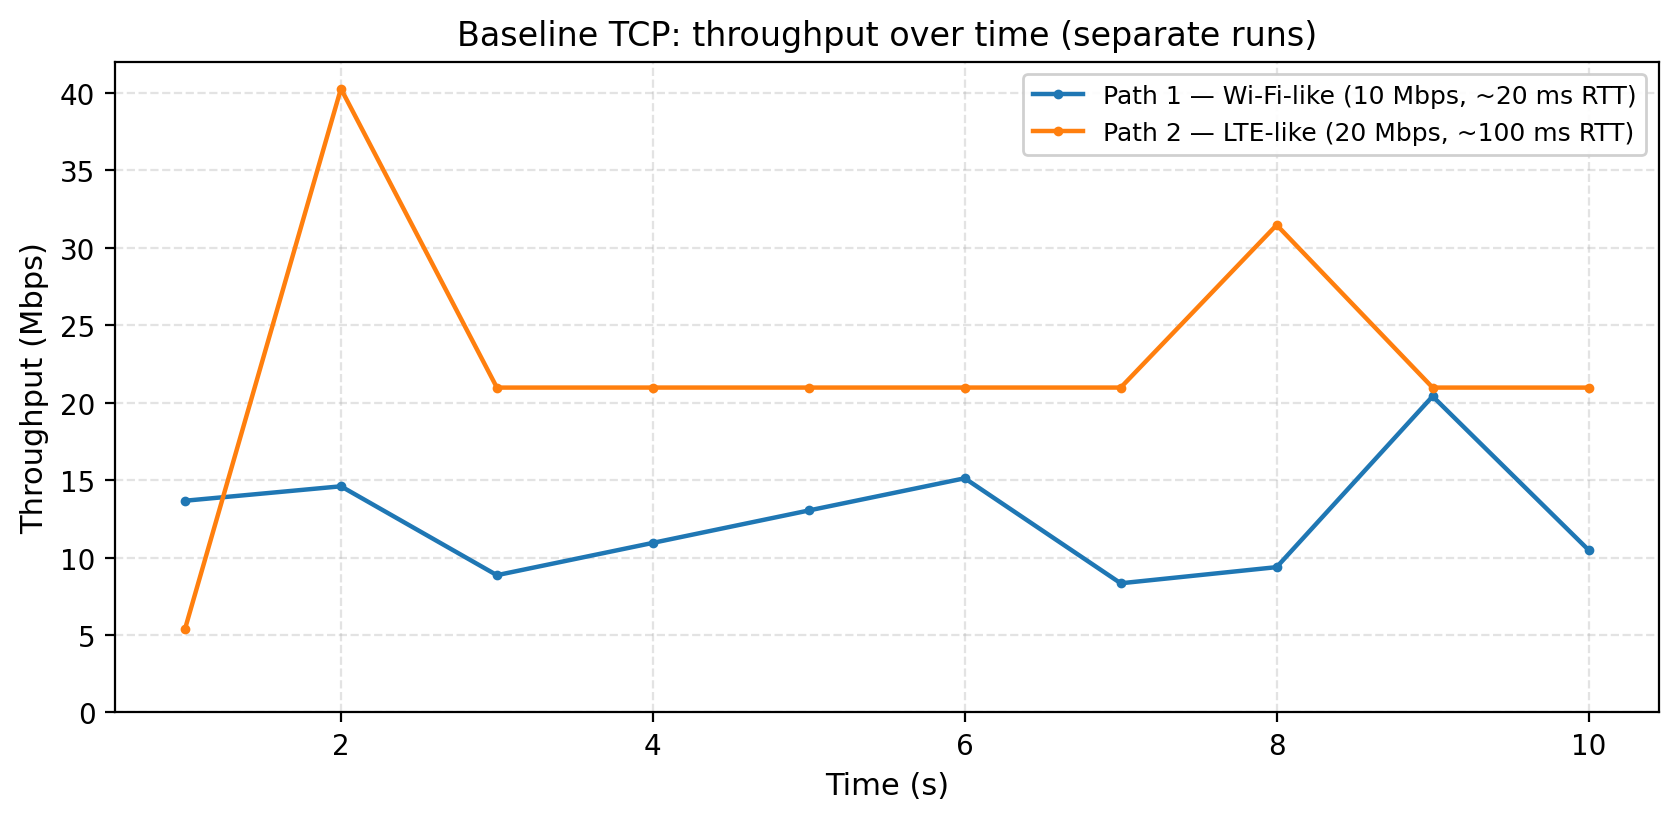
\includegraphics[width=0.92\linewidth]{fig01_tcp_baseline_timeseries.png}
  \caption{Experiment~1: per-second throughput for sequential single-path TCP runs (two separate \texttt{iperf3} sessions).}
  \label{fig:exp1}
\end{figure}

\subsection{Experiment~2: TCP baselines vs.\ dual-path aggregation}
Sequential TCP baselines on the heterogeneous topology yield 9.45 and 16.99~Mb/s (combined nominal sum $26.44$~Mb/s). With two concurrent flows (one per interface), we observe per-path averages of 9.49 and 17.67~Mb/s and a reported combined average of 27.16~Mb/s, i.e.\ $\approx$102.7\% ``aggregation efficiency'' relative to the sum of independent TCP measurements---consistent with statistical variation and Mininet timing rather than a protocol violation. Figure~\ref{fig:exp2} contrasts per-path TCP time series with the parallel-stream run.

\begin{figure}[htbp]
  \centering
  \begin{subfigure}[b]{0.92\linewidth}
    \centering
    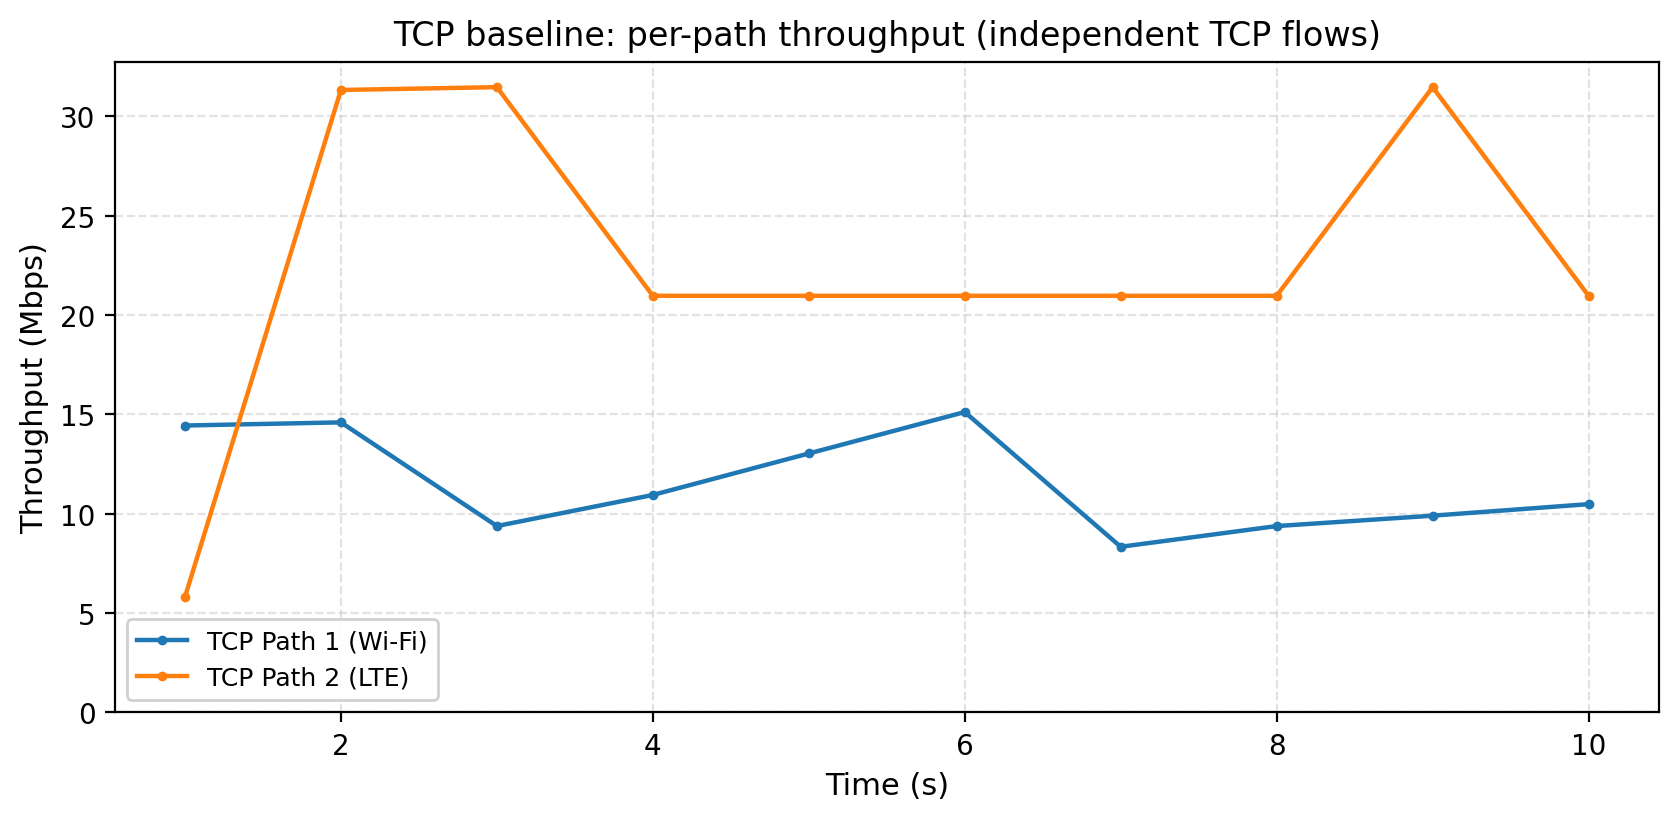
\includegraphics[width=\linewidth]{fig02_tcp_baseline_timeseries.png}
    \caption{Sequential TCP baselines (one path at a time).}
  \end{subfigure}

  \vspace{0.6em}
  \begin{subfigure}[b]{0.92\linewidth}
    \centering
    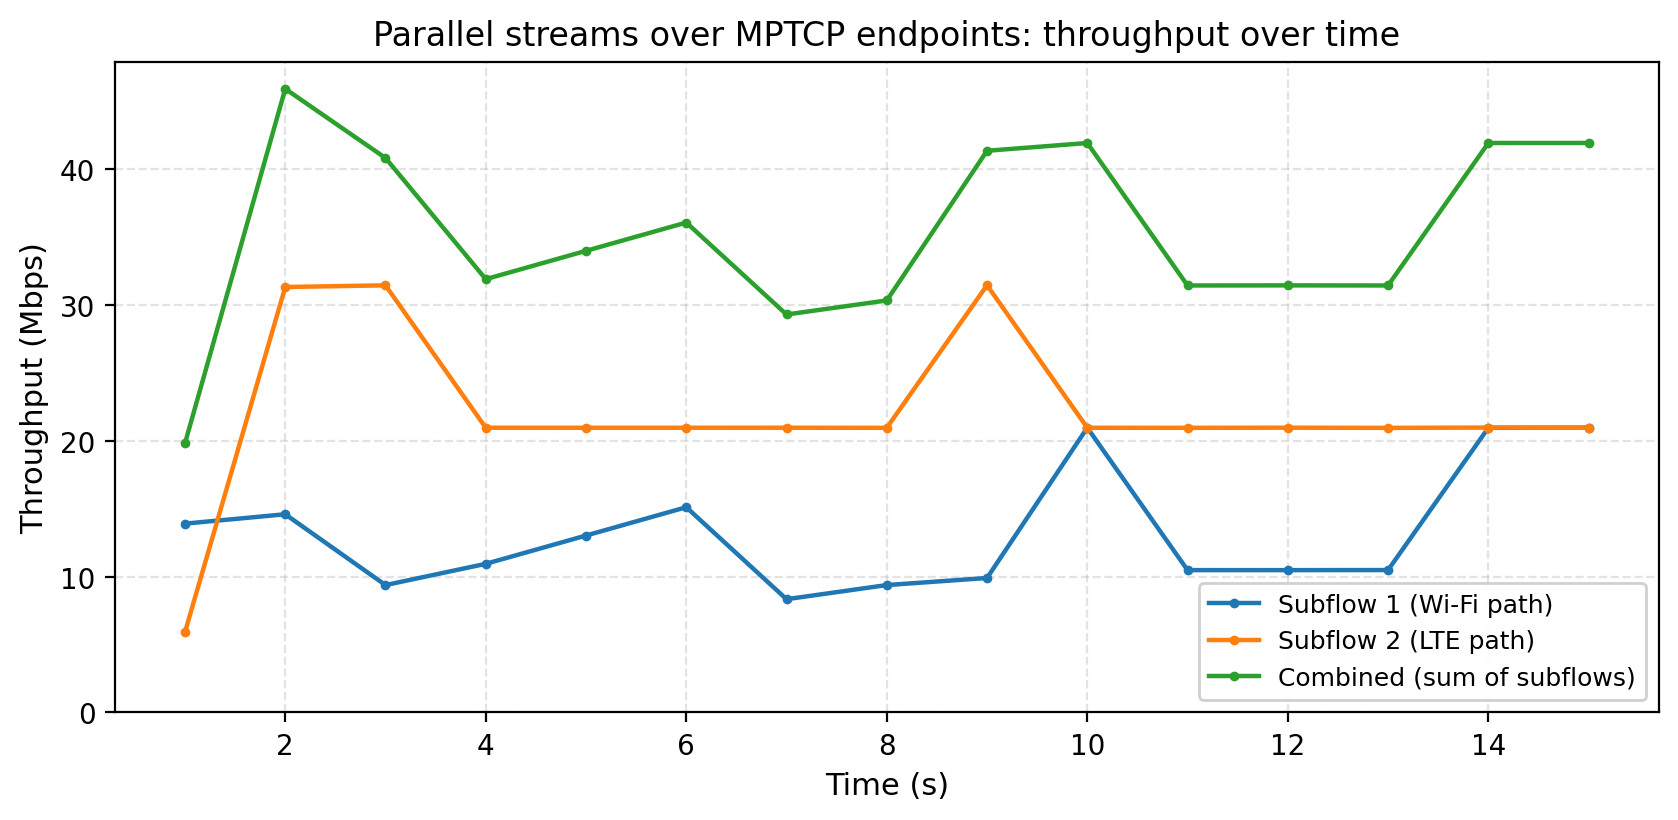
\includegraphics[width=\linewidth]{fig02_mptcp_parallel_streams_timeseries.png}
    \caption{Parallel \texttt{iperf3} streams, one bound to each interface (MPTCP endpoints enabled).}
  \end{subfigure}
  \caption{Experiment~2: throughput over time for baselines vs.\ dual-path aggregation.}
  \label{fig:exp2}
\end{figure}

\subsection{Experiment~3: Sudden path failure}
At $t=10$~s the receiver's first-path interface is taken down and the corresponding client is stopped. The LTE-side stream continues for the full 30~s window with average throughput 18.37~Mb/s and zero retransmissions on that stream in our log, while the Wi-Fi stream shows throughput dropping to zero after the failure. This supports \textbf{session continuity} in the sense that the application-level transfer on the surviving path need not be restarted; aggregate goodput, however, falls to single-path levels after the event. Figure~\ref{fig:exp3} marks the failure instant on the combined throughput trace.

\begin{figure}[htbp]
  \centering
  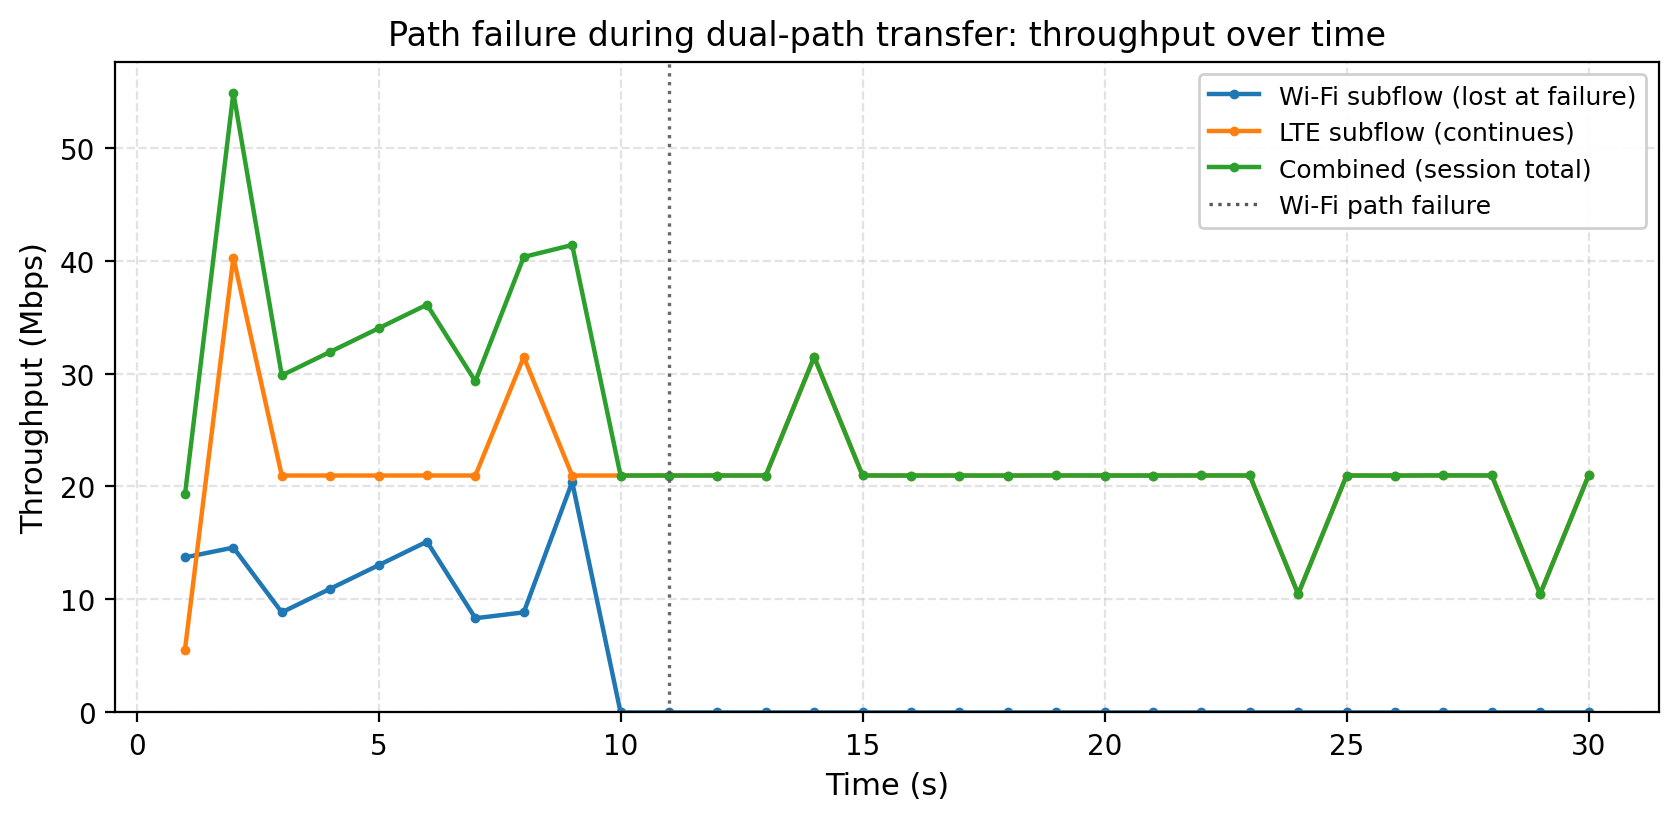
\includegraphics[width=0.92\linewidth]{fig03_path_failure_throughput.png}
  \caption{Experiment~3: combined throughput with vertical line at path failure ($t=10$~s).}
  \label{fig:exp3}
\end{figure}

\subsection{Experiment~4: Bandwidth collapse on one path}
Path~1 and Path~2 each start at 10~Mb/s and $\approx$40~ms RTT. Dual-stream baselines achieve combined $\approx$18.76~Mb/s, slightly above the sum of independent TCP baselines (18.56~Mb/s), matching the printed 101.1\% aggregation efficiency. After Path~2 is throttled to 2~Mb/s at $t=10$~s, the driver's windowed averages report combined throughput falling from $\approx$24.51~Mb/s before collapse to $\approx$15.33~Mb/s after, i.e.\ \textbf{62.5\% retained}. Path~1's average rises from $\approx$12.25 to $\approx$13.71~Mb/s in the post-collapse window, indicating load shifting toward the stable path; Path~2 shows many retransmissions (1863 over 25~s in our log) as congestion control reacts to the bottleneck. Figure~\ref{fig:exp4} contrasts the pre-collapse aggregation shape with the collapse scenario.

\begin{figure}[htbp]
  \centering
  \begin{subfigure}[b]{0.92\linewidth}
    \centering
    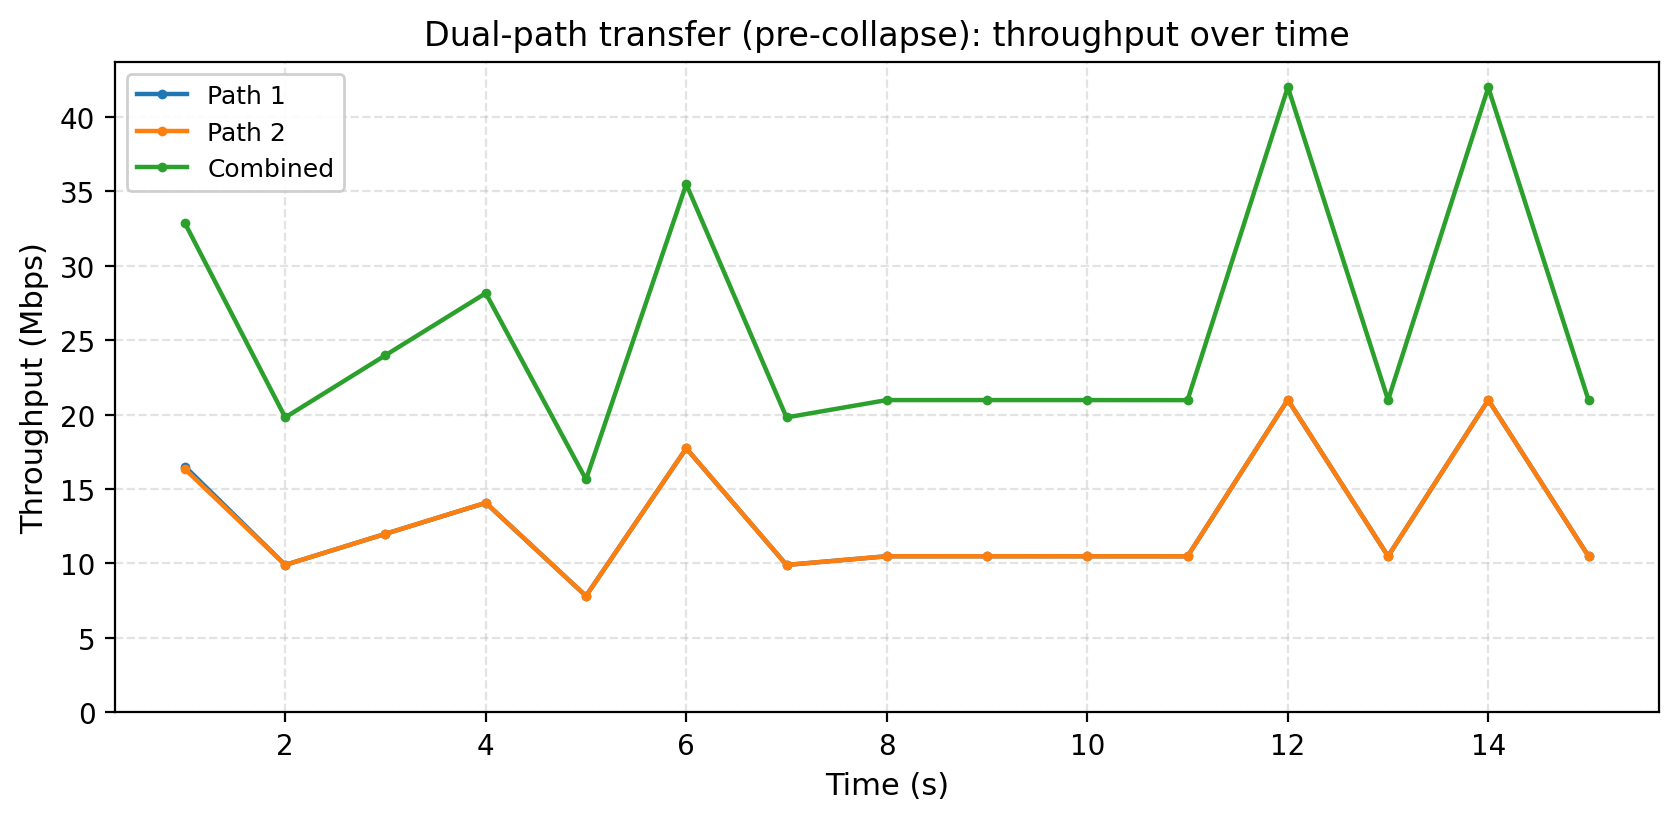
\includegraphics[width=\linewidth]{fig04_mptcp_baseline_timeseries.png}
    \caption{Dual-path baseline before any impairment.}
  \end{subfigure}

  \vspace{0.6em}
  \begin{subfigure}[b]{0.92\linewidth}
    \centering
    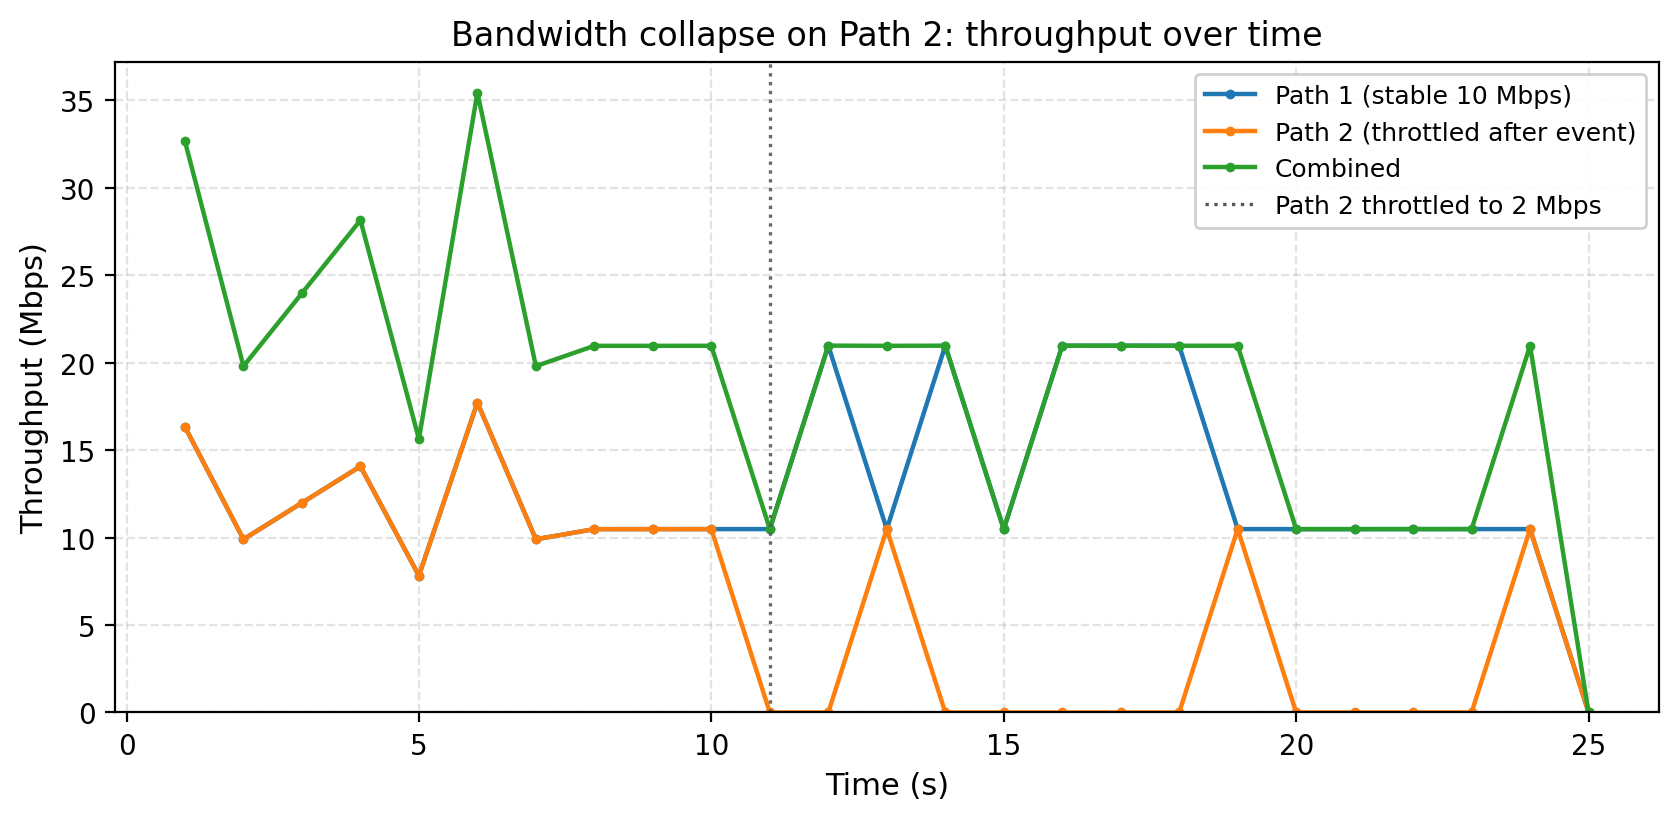
\includegraphics[width=\linewidth]{fig04_bandwidth_collapse_timeseries.png}
    \caption{Dual-path run with Path~2 throttled to 2~Mb/s at $t=10$~s (marker in plot).}
  \end{subfigure}
  \caption{Experiment~4: symmetric topology---baseline vs.\ bandwidth collapse on Path~2.}
  \label{fig:exp4}
\end{figure}

\subsection{Experiment~5: RTT spike on Path~2}
Injecting $\approx$800~ms RTT on Path~2 at $t=10$~s while using TCP \emph{only} on Path~2 reduces average throughput for that run to 4.22~Mb/s, with before/after spike window averages of 11.93 and 1.61~Mb/s (13.5\% throughput retained on that single path). Under dual-path transfer, combined throughput retained across the same event is reported as \textbf{71.0\%} (23.85~Mb/s before vs.\ 16.94~Mb/s after), with Path~2's post-spike average dropping to 4.03~Mb/s while Path~1 increases modestly (11.92 to 12.91~Mb/s). Figure~\ref{fig:exp5a} shows the multipath time series; Figure~\ref{fig:exp5b} summarizes the TCP vs.\ MPTCP comparison from the driver's final table.

\begin{figure}[htbp]
  \centering
  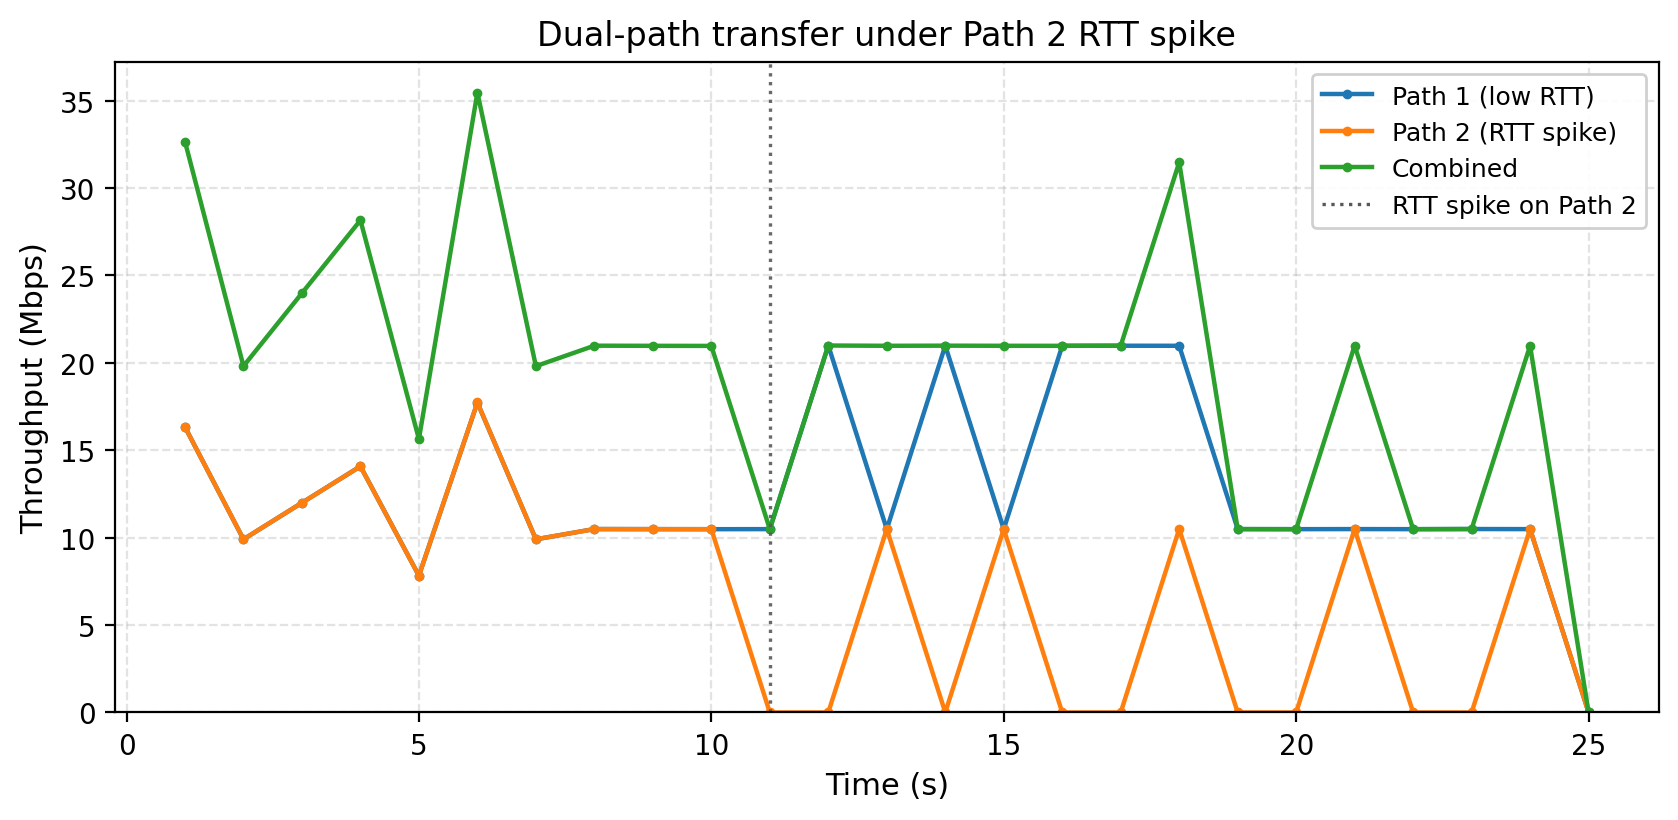
\includegraphics[width=0.92\linewidth]{fig05_mptcp_rtt_spike_timeseries.png}
  \caption{Experiment~5: per-path and combined throughput during Path~2 RTT spike (dual streams).}
  \label{fig:exp5a}
\end{figure}

\begin{figure}[htbp]
  \centering
  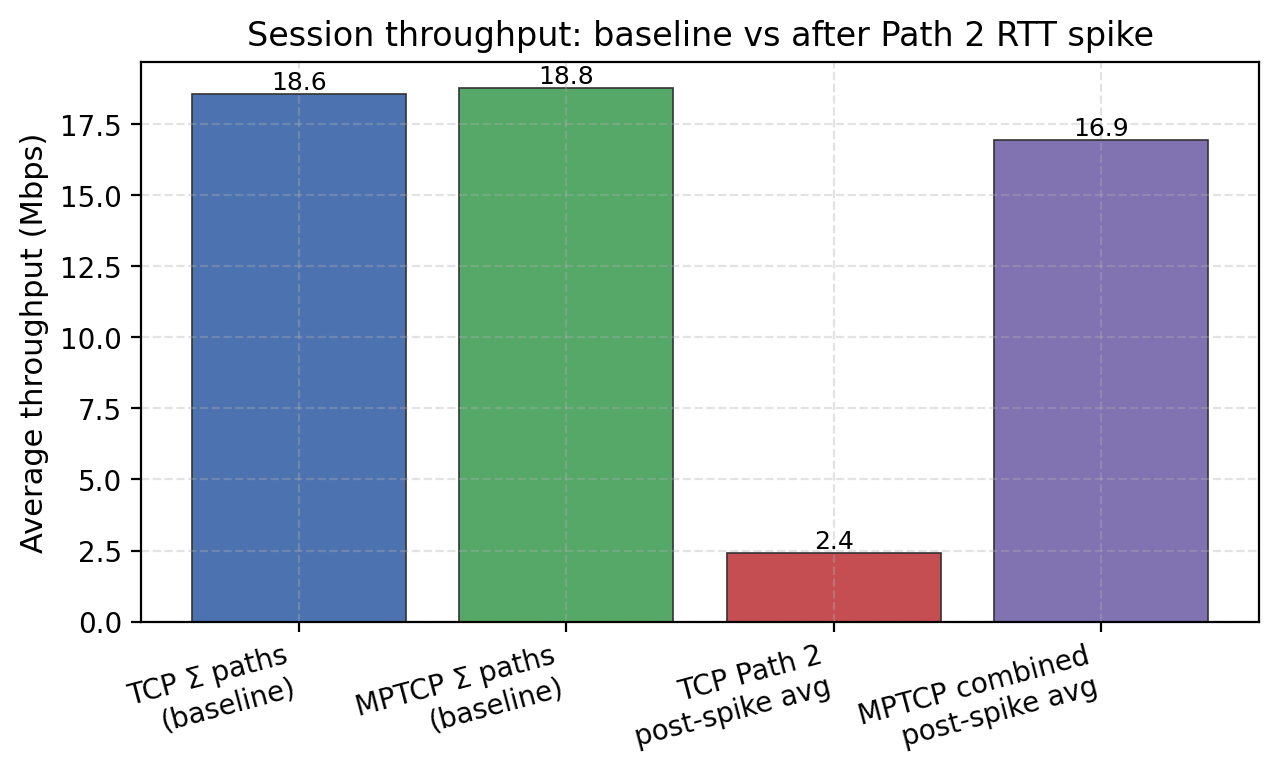
\includegraphics[width=0.75\linewidth]{fig05_summary_post_spike_comparison.png}
  \caption{Experiment~5: summary comparison (throughput retained under spike; TCP single-path vs.\ multipath-style aggregate).}
  \label{fig:exp5b}
\end{figure}

\begin{table}[htbp]
  \centering
  \caption{Experiment~5: selected metrics from the automated summary table (post-spike windows).}
  \label{tab:exp5}
  \begin{tabular}{lc}
    \toprule
    Metric & Value \\
    \midrule
    TCP Path~2 only --- avg.\ during full 25~s run & 4.22~Mb/s \\
    TCP Path~2 only --- throughput retained (post-spike window) & 13.5\% \\
    MPTCP-style dual stream --- combined throughput retained & 71.0\% \\
    Ratio: MPTCP combined avg.\ vs.\ TCP Path~2 only (driver table) & $\approx 10.5{\times}$ \\
    \bottomrule
  \end{tabular}
\end{table}

\subsection{Experiment~6: Handover stress (primary-path RTT ramp)}
\label{subsec:exp6}

This run (\texttt{6.py}, log \texttt{Outputs/6.txt}) uses two $10$~Mb/s paths with Path~1 initially lower RTT ($20{+}20$~ms per link on \texttt{TCLink}) and Path~2 higher RTT ($50{+}50$~ms), analogous to a ``Wi-Fi'' vs.\ ``LTE'' preference. Kernel MPTCP uses the \texttt{blest} packet scheduler. Part~1--2 repeat TCP per-path baselines and a $15$~s dual-stream aggregation baseline. Part~3 runs parallel streams for $25$~s; after $t=10$~s, Path~1 one-way delay is stepped upward via \texttt{tc netem} on host interfaces and \texttt{s1} ports (target RTT milestones $100$--$250$~ms) so the stack should shift traffic toward Path~2. \textbf{No matplotlib figure} was produced for this script; we rely on the driver's summary and the per-second table below.

Table~\ref{tab:exp6baseline} gives baselines; Table~\ref{tab:exp6handover} summarizes the handover phase. Combined average throughput changes only slightly across the event boundary ($24.89$~Mb/s before vs.\ $23.39$~Mb/s after), while Path~1's average in those windows falls from $11.94$ to $10.49$~Mb/s and Path~2's post-handover average is $12.91$~Mb/s---consistent with modest load migration. Path~1 accumulated $493$ retransmissions over the $25$~s handover run (Path~2: $0$ in our log), reflecting congestion dynamics on the degraded path. The per-second trace shows a short dip at $t{=}12$~s (Path~1 reported $0$~Mb/s, total $10.49$~Mb/s) before recovery, illustrating transient rebalancing rather than a hard failure.

\begin{table}[htbp]
  \centering
  \caption{Experiment~6: TCP baselines and dual-stream aggregation (from \texttt{Outputs/6.txt}).}
  \label{tab:exp6baseline}
  \begin{tabular}{lcc}
    \toprule
    Phase & Quantity & Value \\
    \midrule
    \multirow{3}{*}{TCP (10~s each)} & Path~1 avg & 9.28~Mb/s \\
     & Path~2 avg & 8.68~Mb/s \\
     & Sum (theoretical cap $\sim$20~Mb/s) & 17.97~Mb/s \\
    \midrule
    \multirow{4}{*}{Dual-stream baseline (15~s)} & Path~1 avg & 9.38~Mb/s \\
     & Path~2 avg & 8.98~Mb/s \\
     & Combined avg & 18.36~Mb/s \\
     & Aggregation efficiency vs.\ TCP sum & 102.2\% \\
    \bottomrule
  \end{tabular}
\end{table}

\begin{table}[htbp]
  \centering
  \caption{Experiment~6: handover run ($25$~s; Path~1 RTT stepped after $t{=}10$~s). Combined averages are windowed by the driver.}
  \label{tab:exp6handover}
  \begin{tabular}{lc}
    \toprule
    Metric & Value \\
    \midrule
    Combined throughput avg.\ \emph{before} handover window & 24.89~Mb/s \\
    Combined throughput avg.\ \emph{after} handover window & 23.39~Mb/s \\
    Path~1 avg before / after (driver windows) & 11.94 / 10.49~Mb/s \\
    Path~2 avg after handover (driver) & 12.91~Mb/s \\
    Path~1 / Path~2 avg over full $25$~s run & 9.27 / 9.20~Mb/s \\
    Retransmissions (Path~1 / Path~2) & 493 / 0 \\
    \bottomrule
  \end{tabular}
\end{table}

\begin{table}[htbp]
  \centering
  \caption{Experiment~6: excerpt of per-second combined throughput (Mb/s) around the handover (from log).}
  \label{tab:exp6timeseries}
  \begin{tabular}{crrr}
    \toprule
    $t$ (s) & Path~1 & Path~2 & Total \\
    \midrule
    8 & 10.48 & 10.49 & 20.97 \\
    9 & 10.49 & 10.49 & 20.97 \\
    10 & 10.48 & 10.48 & 20.97 \\
    11 & 10.49 & 10.49 & 20.98 \\
    12 & 0.00 & 10.49 & 10.49 \\
    13 & 10.49 & 20.99 & 31.48 \\
    14 & 10.49 & 10.48 & 20.97 \\
    15 & 10.49 & 10.48 & 20.97 \\
    \bottomrule
  \end{tabular}
\end{table}

Overall, path failure and RTT-spike experiments show the qualitative benefit of maintaining a second usable path: aggregate throughput degrades but the transfer is not confined to the impaired link alone. Experiment~6 complements this by showing that gradual primary-path degradation can be absorbed with limited aggregate loss, at the cost of retransmissions on the degrading path.



\section{Conclusion}
\label{sec:conclusion}

We built a Mininet-based harness to compare single-path TCP with a multipath-capable Linux configuration under emulated mobility stressors. Independent TCP baselines track configured link capacities well (Experiment~1). Running two interface-bound \texttt{iperf3} flows shows that both emulated paths can be utilized together, with combined throughput matching or slightly exceeding the sum of sequential baselines in our logs (Experiment~2). A hard interface failure on one path stops that subflow immediately, but the surviving path continues delivering throughput without restarting the server (Experiment~3), which is the operational notion of continuity we could measure. Bandwidth collapse on one path reduces aggregate throughput but the stable path absorbs additional load, recovering a substantial fraction of the pre-event aggregate (62.5\% retained in Experiment~4). An RTT spike on a single path devastates that TCP flow (13.5\% retained on Path~2 alone), whereas the dual-path setup retains 71.0\% of its pre-spike combined average (Experiment~5). Experiment~6 steps up delay on the initially preferred path: aggregate throughput before and after the handover window differs only modestly ($24.89$ vs.\ $23.39$~Mb/s in our log), with Path~1 incurring most retransmissions---consistent with gradual load shift under scheduler control rather than catastrophic outage.

These results support the intuition behind MPTCP in heterogeneous access: spare paths provide redundancy against localized impairment. Our study does not yet quantify Jain fairness across competing flows; parallel \texttt{iperf3} clients remain an approximation of full multipath socket behavior in every scenario---so claims should be read as emulator-scoped evidence rather than universal WAN performance.

\section{Future Work}
\label{sec:future}

\textbf{Competing-flow fairness.} The project brief also mentions fairness when multiple independent flows contend for the same paths. A natural extension is to add background \texttt{iperf3} or UDP cross-traffic and report Jain's fairness index or relative throughput ratios, optionally with a dedicated figure.

\textbf{Other extensions.} Wire Experiment~6 to \texttt{plot\_helpers} for a publication-style time series. Compare additional kernel schedulers (\texttt{redundant}, \texttt{default}) side by side with \texttt{blest}. Longer runs with repeated handovers and explicit address handover signaling (\texttt{ip mptcp endpoint}) would tighten the mobility story. Adding ping or \texttt{ss -ti} statistics would connect throughput traces to measured RTT and retransmission behavior more directly.

\newpage
\bibliographystyle{unsrtnat}
\bibliography{mybib}
\vspace{2mm}

% \newpage

% \subsection{Related Work}
% \input{Main_Matter/JOI/Interoperability/interop_related_work}

% \bibliographystyle{unsrt}
% \bibliography{Main}

%\normalsize

%\newpage
%\vspace{15 mm}
%\noindent {\bf {\Huge APPENDICES}}

%\appendix
%\input{Main_Matter/Appendices/Appendix1.tex}

%\newpage
%\input{Appendix2.tex}
\end{singlespace}
\end{document}
